\documentclass[10pt,letterpaper,conference,compsoc,oneside]{IEEEtran}
\usepackage[utf8]{inputenc}
\usepackage{amsmath}
\usepackage{amsfonts}
\usepackage{amssymb}
\usepackage{amsthm}

%% --------------------------------------------
%% packages
%% --------------------------------------------
\usepackage{xspace}
\usepackage[ngerman, english]{babel}
\usepackage{url}
\usepackage{algorithm}
\usepackage[noend]{algpseudocode}
\usepackage{pgfplots}
\usepackage{booktabs}
\usepackage{hyperref}

%% --------------------------------------------
%% bibliography preamble
%% --------------------------------------------
\usepackage[natbib=true,style=ieee,backend=biber,urldate=long]{biblatex}
\addbibresource{report.bib}

%% --------------------------------------------
%% commands
%% --------------------------------------------
\newcommand{\etal}{~et~al.\xspace}
\newcommand{\ie}{i.e.\xspace}
\newcommand{\eg}{e.g.\xspace}

%% --------------------------------------------
%% theorems and environments
%% --------------------------------------------
\theoremstyle{definition}
\newtheorem{definition}{Definition}[section]

%% --------------------------------------------
%% todo's
%% --------------------------------------------
\usepackage[colorinlistoftodos, textwidth=1cm]{todonotes} % add ",disable" in [] to remove all todos, missing figures and the todo list
\newcommand{\todoEmpty}[2][]{\todo[inline, #1]{#2}}
\newcommand{\todoMissing}[2][]{\todoEmpty[color=magenta!80, linecolor=magenta!80, #1]{Missing: #2}}
\newcommand{\todoCheck}[2][]{\todoEmpty[color=red!80, linecolor=red!80, #1]{Check: #2}}
\newcommand{\todoRevise}[2][]{\todoEmpty[color=orange!80, linecolor=orange!80, #1]{Revise: #2}}
\newcommand{\todoCitation}[2][]{\todoEmpty[color=yellow!80, linecolor=yellow!80, #1]{Citation: #2}}
\newcommand{\todoLanguage}[2][]{\todoEmpty[color=blue!40!white, linecolor=blue!40!white, #1]{Language: #2}}
\newcommand{\todoQuestion}[2][]{\todoEmpty[color=green!80!white, linecolor=green!80!white, #1]{Question: #2}}
\newcommand{\todoNote}[2][]{\todoEmpty[color=black!20!white, linecolor=black!20!white, #1]{Note: #2}}
\newcommand{\todoFigure}[5]{\begin{figure}[#1]\centering\missingfigure[figwidth=#2]{#3}\caption{#4}\label{#5}\end{figure}}

\begin{document}
%% --------------------------------------------
%% title information
%% --------------------------------------------
\title{Reconstruction of Partial Femurs Using Statistical Shape Models \\ \large{Project Report}}
\author{
	\IEEEauthorblockN{Ferdinand~Badenberg\IEEEauthorrefmark{1} and Clemens~Büchner\IEEEauthorrefmark{2}}
	\IEEEauthorblockA{
		University of Basel\\
		Department~of~Mathematics~and~Computer~Science\\
		Email:~\IEEEauthorrefmark{1}\href{mailto:ferdinand.badenberg@unibas.ch}{ferdinand.badenberg@unibas.ch}, \IEEEauthorrefmark{2}\href{mailto:clemens.buechner@unibas.ch}{clemens.buechner@unibas.ch}
}}
\maketitle
\IEEEaftertitletext{\vspace{-1\baselineskip}}

%% --------------------------------------------
%% abstract
%% --------------------------------------------
\begin{abstract}
	Part of the statistical shape modelling course on Future Learn is the challenge to reconstruct femur bones from partial data using given training data. 
This problem has important real world applications in the medical field. 
While the procedure itself is straightforward, obtaining a good model to predict the reconstructions with a high accuracy can be challenging. 
In the following, we will present our strategies, struggles and solutions for this problem.
\end{abstract}

%% --------------------------------------------
%% main part of the paper
%% --------------------------------------------
\section{Introduction}
\label{sec:intro}

\todoRevise{review introduction (looks good -F)}

Being able to reconstruct shapes from partial representations is a useful tool in medical applications.
For example, one could be interested in the original shape of remaining parts of a bone fracture, which enables building suitable artificial implants.
Many more similar fields of applications could be imagined.
However, in this paper we only consider the specific problem of reconstructing femur bones from partial femur shapes.

Knowing typical characteristics of the underlying shape is essential to estimating a high-quality reconstruction.
It can be learned from complete data of the corresponding shape families.
We call the result of this learning process a \emph{statistical shape model}.

This paper reports our findings from the project posed in the Future Learn course called ``Statistical Shape Modelling: Computing the Human Anatomy''~\cite{mooc2019statistical}.
The most part of the theory used is also acquired from that course.

\section{Background}
\label{sec:background}

This section provides some fundamental knowledge required to understand our implementations described in Section~\ref{sec:methods}.
However, the theory will only be covered broadly, as it is described in-depth in the corresponding online course~\citep{mooc2019statistical}.

%% --------------------------------------------

\subsection{Gaussian Process}
\label{subsec:gp}

\todoCheck{double citation intentional?}
According to \citeauthor{seeger2004gaussian}~\cite{seeger2004gaussian}, ``Gaussian processes (GPs) are natural generalisations of multivariate Gaussian random variables to infinite [\dots] index sets.''
A GP is fully defined by a mean function $ \mu : \Omega \rightarrow \mathbb{R}^n $ and a covariance function $k : \Omega \times \Omega \rightarrow \mathbb{R}^{n \times n} $, where $\Omega$ is the domain and $n$ the dimensionality of the data~\citep{mooc2019statistical}.

\todoRevise{Might be incomplete. (Looks good -F)}

%% --------------------------------------------

\subsection{Statistical Shape Model}
\label{subsec:ssm}

By analyzing a dataset of shapes from the same shape family we can build a statistical shape model (SSM).
We assume that the variations in the available shapes originate in a set of normally distributed features.
For each shape in the dataset, the deformation field to a corresponding reference shape is computed.
From the deformation vectors, we can calculate the mean shape as well as a covariance matrix.
With these, we can fully describe all shapes from the dataset as well as many more similar shapes.

%% --------------------------------------------

\subsection{Distance Metrics}
\label{subsec:metrics}

We estimate the accuracy of our model using two different distance measures.
They evaluate the difference between two meshes.
Both metrics are also used for evaluating the final reconstructions in the SICAS competition~\cite{smir}.
\todoCheck{Smir/sicas was not yet introduced, move to \autoref{subsec:recon}?}

\paragraph{Average Distance}
The average distance computes the average over all distances from every point on one mesh to its closest point on the other mesh:
$$ \frac{1}{|M_1|} \sum_{p \in M_1} \mathit{dist}_{M_2}(p) $$
where $p \in M_1$ denotes a point $p$ on mesh $M_1$ and $\mathit{dist}_{M_2}$ is a function mapping a point to its minimal distance to mesh~$M_2$.

\paragraph{Hausdorff Distance}
Unlike the average distance, this metric computes the difference between two meshes in both directions.
Two shapes are said to be close to each other, if the Hausdorff distance is low.
The distance is calculated as follows~\cite{hausdorff}:
$$ \max \left\{ \begin{array}{ll}
  \sup_{p_1 \in M_1} \inf_{p_2 \in M_2} \mathit{dist}(p_1, p_2), \\
  \sup_{p_2 \in M_2} \inf_{p_2 \in M_2} \mathit{dist}(p_1, p_2) 
\end{array}\right\}. $$
Informally, it describes the maximum over all shortest distances from each point on either mesh to get to the other mesh.

\section{Methods}
\label{sec:methods}

In the following sections we describe the methods used for our approach.

%% --------------------------------------------

\subsection{Landmarks}
\label{subsec:landmarks}

We have manually clicked ten landmarks on each femora instance: model and CT images.
All landmarks lie on prominent parts of the bone, such as the condyles or trochanters.
These are easily recognizable even if the ground truth is unavailable.
They are to be found as first occurrence of tissue when sliding through cuts of the bone in either $x$, $y$, or $z$-direction. 
We have used 6 landmarks on the lower part and 4 landmarks on the femur head.

%% --------------------------------------------

\subsection{Markov Chains}
\label{subsec:markovchains}

Our approach uses three Markov chains sequentially. 
Each of them does 5000 iterations passing the best sample according to an ASM evaluator as initial sample to the subsequent chain.

For the first one, we used our manually clicked landmarks together with a shape likelihood evaluator.
While the second chain favors proposals with a larger step size, the third tries to improve the fit with smaller changes.

We used and tested different combinations of mixture proposals consisting of shape update, rotation, and translation proposals. 
The parameters of our final proposals can be found in \autoref{tbl:proposals}. 
In \autoref{tbl:markovchains} we show the probability of choosing each proposal in the mixture proposals.

\begin{table}
  \centering
  \caption{Proposals used by our Markov Chains}
  \label{tbl:proposals}
  \begin{tabular}{lr}
    \toprule
      \textbf{Update Proposal} &
      Standard Deviation \\
    \midrule
      Tiny Shape & 0.02 \\
      Small Shape & 0.05 \\
      Medium Shape & 0.10 \\
      Large Shape & 0.30 \\
      Rotation & 0.01 \\
      Translation & 1.00 \\
    \bottomrule
  \end{tabular}
\end{table}

\begin{table}
  \centering
  \caption{Weight combinations of proposals for the Markov Chains}
  \label{tbl:markovchains}
  \begin{tabular}{lrrr}
    \toprule
      \textbf{Update Proposal} &
      Chain 1 &
      Chain 2 &
      Chain 3 \\
    \midrule
      Tiny Shape & - & 0.00 & 0.20 \\
      Small Shape & 0.10 & 0.30 & 0.50 \\
      Medium Shape & 0.20 & 0.40 & 0.20 \\
      Large Shape & 0.10 & 0.10 & - \\
      Rotation & 0.30 & 0.10 & 0.05 \\
      Translation & 0.30 & 0.10 & 0.05 \\
    \bottomrule
  \end{tabular}
\end{table}

\section{Results}
\label{sec:results}

In this section we present the outcome of our implementation.
For testing purposes, we have used 5 images together with their ground truth femur mesh.
We used the average distance and the Hausdorff distance as metrics to evaluate our fitted meshes.
The results of these evaluations can be found in \autoref{tbl:testfit}.

\begin{table}
  \centering
  \caption{Test fit distance to ground truth}
  \label{tbl:testfit}
  \begin{tabular}{lrr}
    \toprule
      \textbf{Bone Image} &
      Average Distance &
       Hausdorff Distance \\
    \midrule
      Bone 4 & 0.57 & 4.98 \\
      Bone 14 & 0.41 & 2.23 \\
      Bone 23 & 0.59 & 3.16 \\
      Bone 25 & 0.71 & 5.24 \\
      Bone 30 & 0.51 & 2.94 \\
    \midrule
      Average & 0.56 & 3.71 \\
      Standard Deviation & 0.11 & 1.33 \\
    \bottomrule
  \end{tabular}
\end{table}

We first optimized the parameters with respect to the test data.
Afterwards, we went on applying the approach to another 5 target images without ground truth.
For these, only a visual evaluation was done, as ground truth is necessary to calculate mesh distances.
One instance of the fitted result can be found in \todoMissing{Add figure and reference}.
No alarming discrepancy from the CT contours was found among all targets.

\section{Discussion}
\label{sec:discussion}

We can evaluate the performance of our approach based on the two main results: the average distance from the test fit to the ground truth data and visually analyzing the images of the test or target fit to the CT image. 

%% --------------------------------------------

\subsection{Likelihood Evaluators}
\label{subsec:evaluators}

Applying multiple Markov chains in sequence was the consequence of a problem faced early in the project.
While very strong at precise fits, ASM struggled with general alignment to the CT image on a larger scale: It would align the model to the nearest occurrences of tissue, even if that was not the corresponding part of the bone contour.
To avoid this local optimum, we introduced the leading Markov chain using landmark correspondence in the likelihood evaluator.
This would get the model align roughly to the bone contour. 

After that, we would follow up with the active shape model evaluator which should then closely fit the model to the contours. 
This approach worked very well in practice. 
The landmark evaluator definitely helped to avoid or break out of local minima while the active shape model helped to get a very close fit.

Both our evaluators are product evaluators including the prior probability either with the landmarks fit or the profiles.
We also tried adding the landmarks evaluator to the product for the second and third chain.
However, this did not lead to any improvement in our result and the change was hence discarded from the final configuration.

%% --------------------------------------------

\subsection{Proposals}
\label{subsec:proposals}

The plan for our proposals was to expand on the idea of multiple sequential Markov chains explained in Section~\ref{subsec:evaluators}: Some of the proposals are more useful during a fitting process on a larger scale while some are better suited for fitting on a small scale. 
We tested a number of different configurations for the parameters involved in the proposals, \ie, the combination of different proposals with different standard deviations. 
The configuration shown in Section~\ref{sec:results} provided the best results among all our experiments. 
Generally, it makes sense to use larger standard deviations early on and set them to continually smaller values. 
Furthermore, we put a larger emphasis on rotation and translation during the first chain and gradually shifted the focus to shape transformations.

%% --------------------------------------------

\subsection{Test Fit}
\label{subsec:testfit}

The average distance results for our test fits are very strong, with an average of 0.56 millimeters. 
We considered this difference to the ground truth to be reasonably small, leading to the conclusion that the procedure worked very well overall. 

When looking at the meshes, we see that one problem that can sometimes occur is that the model gets stuck in a local minimum.
This risk is especially high at parts of the CT image where an adjacent bone is very close to the femur. 
On the left hand side of \autoref{fig:testfit} we see an example where the algorithm converges the true shape, but it is evident that only small variations could move the femur head towards the contour of the pelvis.
The right hand side shows the same fit some slices further on top of the femur head, where the model got stuck in the contour of this adjacent bone.
Further optimization would be necessary to escape such local optima consistently.

\begin{figure}
	\centering
  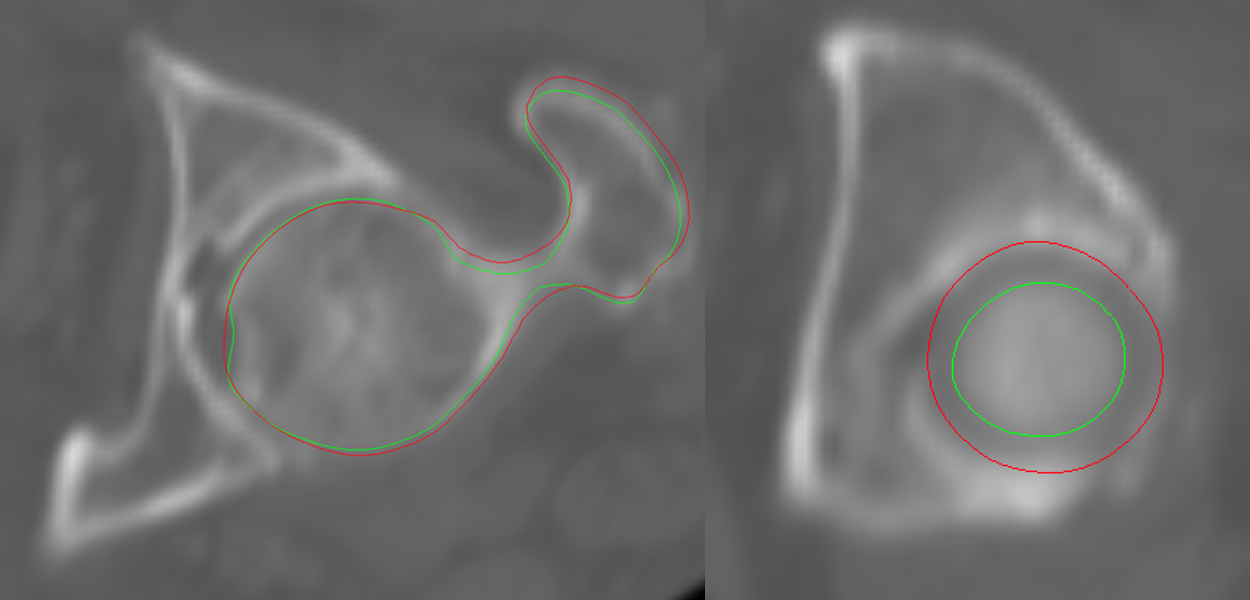
\includegraphics[width=\columnwidth]{./Figures/local_minimum_comparison}
  \caption{
    Two cuts through the image, the fitted model (red) and the ground truth mesh (green).
    On the left, the model successfully escaped the local minimum.
    On the right, it got stuck in a local minimum.
  }
  \label{fig:testfit}
\end{figure}

%% --------------------------------------------

\subsection{Target Fit}
\label{subsec:targetfit}

\todoQuestion{Maybe remove? In my opinion, this does not contribute much to the discussion.}
\autoref{fig:targetfit} shows that the procedure appears to be working for the target CT images as well, as the model is tightly fit to the image contours. An option we considered was to increase the landmark noise variance for this part as we could not double check clicked landmarks on the ground truth mesh, but ultimately, this did not seem necessary due to the many iterations of the procedure afterwards.

\begin{figure}
	\centering
  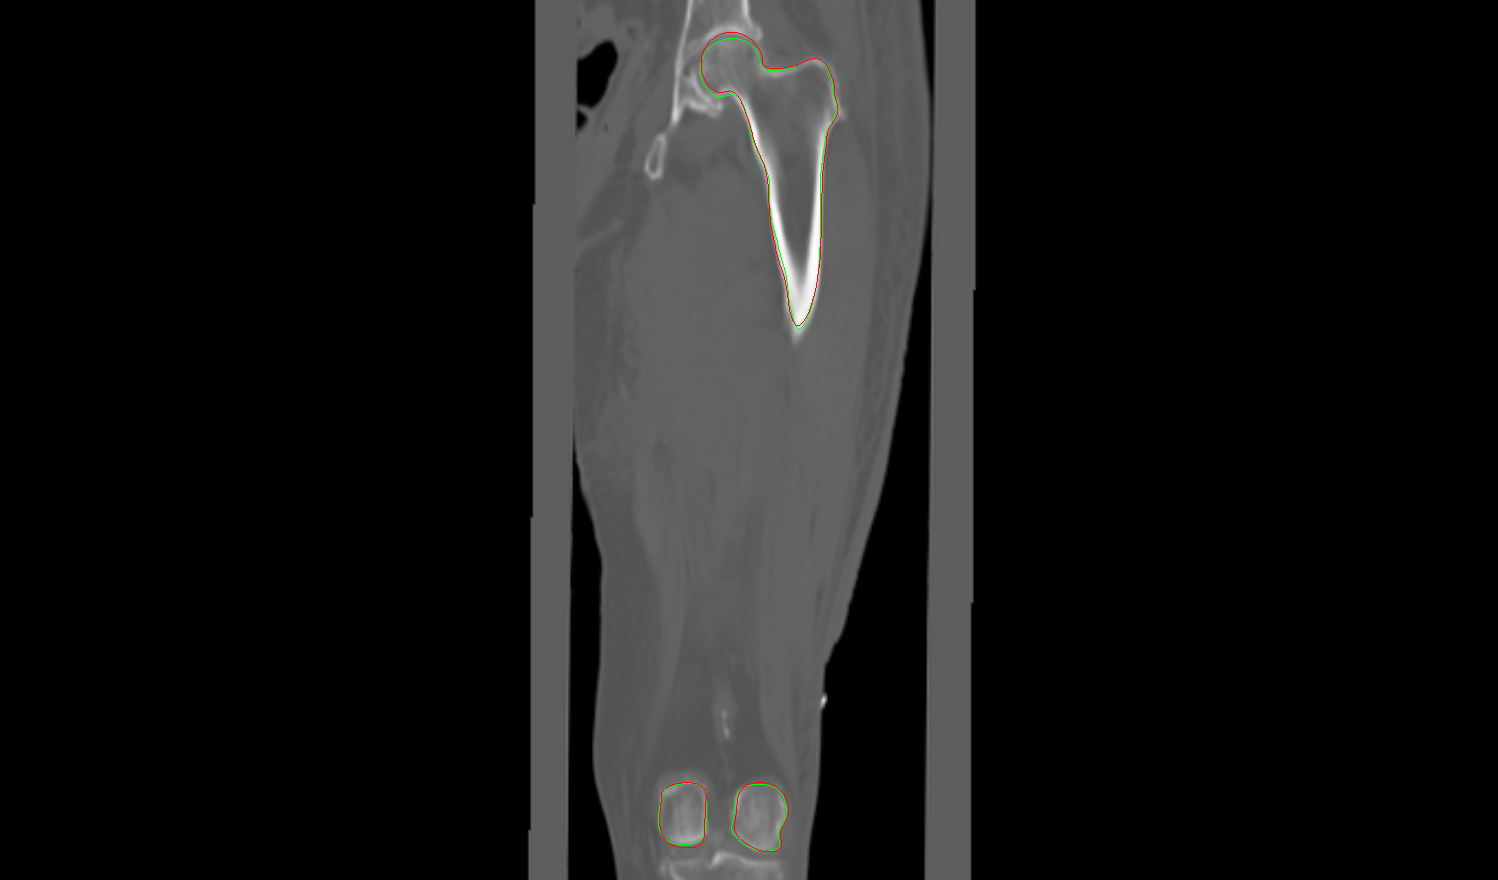
\includegraphics[width=\columnwidth]{./Figures/local_minimum_y-axis}
  \caption{
    Example of a fit of our model to the target CT image. }
  \label{fig:targetfit}
\end{figure}
\todoRevise{Figure with target fit}





\section{Conclusion}
\label{sect:conclusion}

\todoMissing{write conclusion}
\todoMissing{write future work/further improvements}

%% --------------------------------------------
%% bibliography
%% --------------------------------------------
\printbibliography

%% --------------------------------------------
%% appendices
%% --------------------------------------------
% no appendices

\end{document}